\chapter{Pool A --- FR-03: Quên mật khẩu và đặt lại mật khẩu}

\section{Smoke test ban đầu}

Feature có thể truy cập tại \texttt{localhost:5173/forgot-password}. Hai ảnh được
chụp ngày 09/10/2026 lúc 10:31 AM, lần lượt thể hiện bước yêu cầu OTP bằng email
và bước nhập OTP cùng mật khẩu mới. Trạng thái hiện tại là \texttt{Accessible};
chưa có verdict \texttt{Pass/Fail}.

\begin{figure}[H]
  \centering
  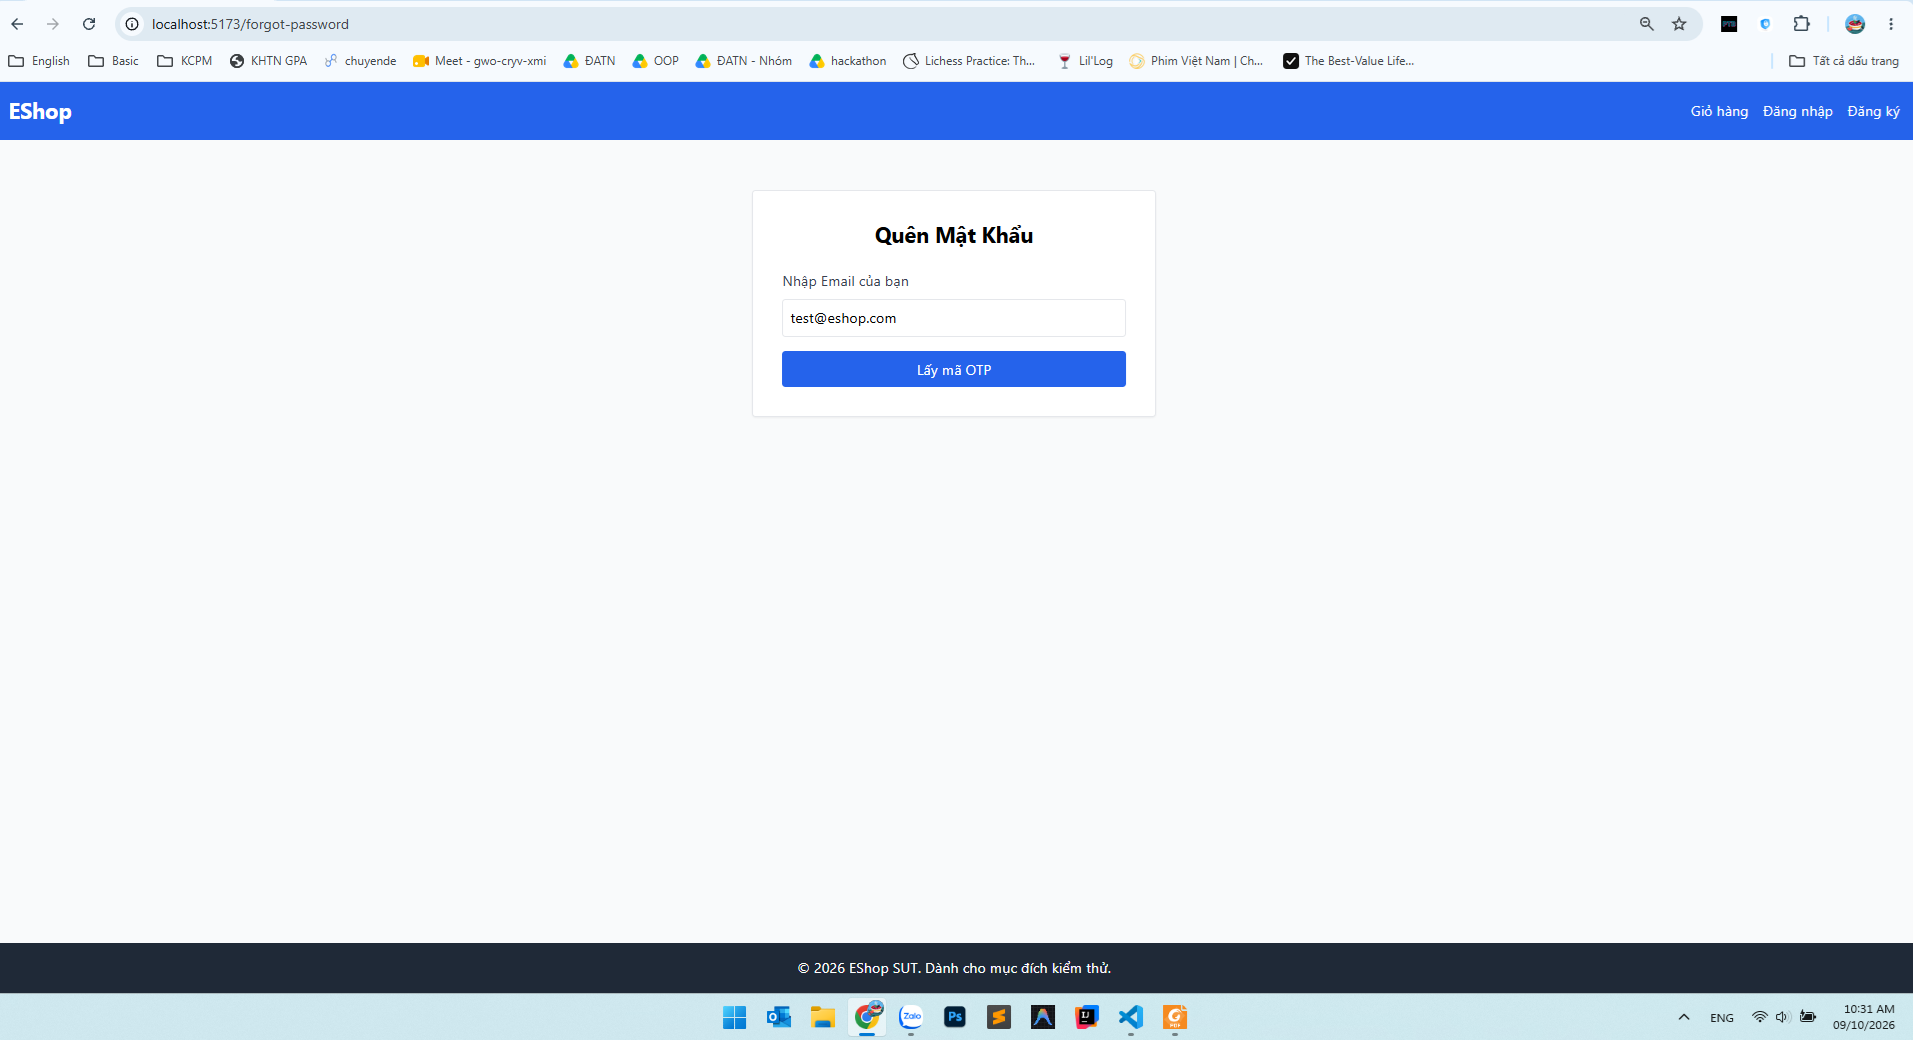
\includegraphics[width=0.96\textwidth]{../../evidence/A/smoke/A-FR03-SMOKE-001-forgot-password.png}
  \caption{A-FR03 --- Màn hình yêu cầu OTP bằng email.}
  \label{fig:a-fr03-forgot-password-smoke}
\end{figure}

\begin{figure}[H]
  \centering
  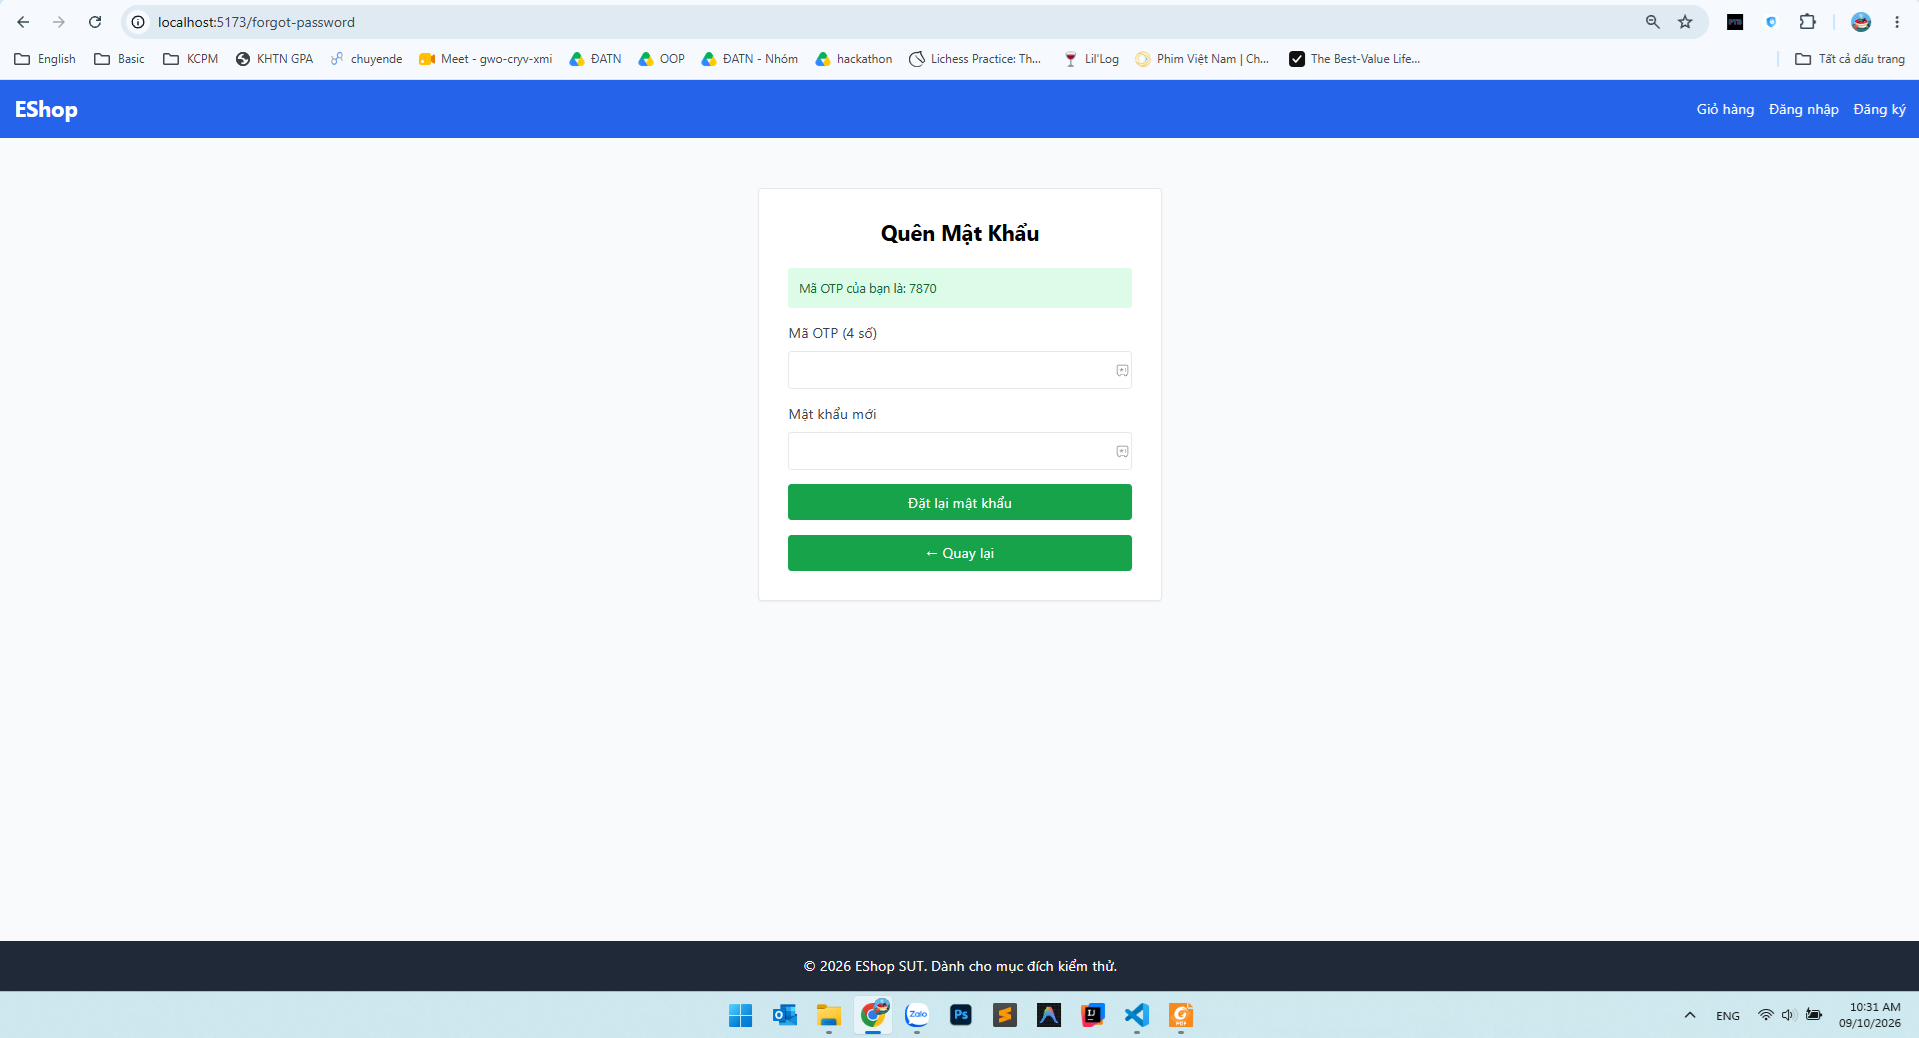
\includegraphics[width=0.96\textwidth]{../../evidence/A/smoke/A-FR03-SMOKE-002-reset-password.png}
  \caption{A-FR03 --- Màn hình nhập OTP và mật khẩu mới.}
  \label{fig:a-fr03-reset-password-smoke}
\end{figure}

Ảnh thứ hai hiển thị OTP \texttt{7870} và nhãn OTP 4 số. Execution chính thức
sau đó xác nhận đây là sai lệch so với yêu cầu OTP 6 chữ số.

\section{Oracle và mô hình miền}

Oracle chính là SRS của dự án. API specification chỉ bổ sung contract
request/response; source code chỉ được dùng để giải thích actual behavior.
Mười bốn rule \texttt{A-R01}--\texttt{A-R14} bao phủ bốn nhóm input:
email, OTP, mật khẩu mới và xác nhận mật khẩu. OTP còn được mô hình hóa theo
value, binding với email và lifecycle.

Equivalence Partitioning được dùng để tách valid/invalid class. Boundary Value
Analysis chọn các điểm gần biên cho OTP length 6, password minimum length 8,
số lượng tối thiểu một chữ hoa, chữ thường, chữ số, allowed special và quan hệ
password--confirm. OTP expiry không thể định lượng vì SRS không cho lifetime;
email length và password maximum cũng không có boundary chính thức.

\begin{table}[H]
  \centering
  \small
  \begin{tabular}{p{0.24\textwidth}p{0.24\textwidth}p{0.36\textwidth}}
    \toprule
    Nhóm & Partition chính & Boundary/quan hệ \\
    \midrule
    Email & Syntax, membership & Không có min/max length \\
    OTP & Format, value, binding, lifecycle & Length 5/6/7; expiry chưa định lượng \\
    Password & Presence, length, composition & Length 7/8/9; count 0/1/2 \\
    Confirm & Empty, exact match, mismatch & Equal; lệch ký tự/case/độ dài \\
    \bottomrule
  \end{tabular}
  \caption{Tóm tắt domain model và boundary của A-FR03.}
\end{table}

\section{Thiết kế và tự động hóa test}

Suite gồm 38 test case: bốn case yêu cầu OTP, 11 case OTP/lifecycle, 13 case
password policy, năm case confirm/security output và năm case GUI. Automation
dùng Playwright với Chrome hệ thống, chạy tuần tự và tự khởi động Web/API khi
cần. SQLite fixture thiết lập precondition, đọc postcondition và khôi phục
password seed/reset token sau lần chạy. Không sửa source SHOP và không gọi API
thay thế cho một procedure được thiết kế là Web end-to-end.

\section{Kết quả thực thi}

\begin{table}[H]
  \centering
  \begin{tabular}{lr}
    \toprule
    Chỉ số & Số lượng \\
    \midrule
    Designed & 38 \\
    Executed & 9 \\
    Passed & 1 \\
    Failed & 8 \\
    Blocked & 29 \\
    Not Run & 0 \\
    \bottomrule
  \end{tabular}
  \caption{Kết quả thực thi A-FR03.}
  \label{tab:a-fr03-result-summary}
\end{table}

\texttt{A-TC-002} là case duy nhất PASS. Tám case FAIL là \texttt{001},
\texttt{003}, \texttt{004} và \texttt{034}--\texttt{038}. Hai mươi chín case
\texttt{005}--\texttt{033} bị chặn vì UI không có trường confirm password;
\texttt{A-TC-014} còn thiếu expiry rule/state/fixture. Do đó execution coverage
chỉ đạt $9/38=23.68\%$ và không thể suy ra feature đã đạt chất lượng yêu cầu.

\begin{figure}[H]
  \centering
  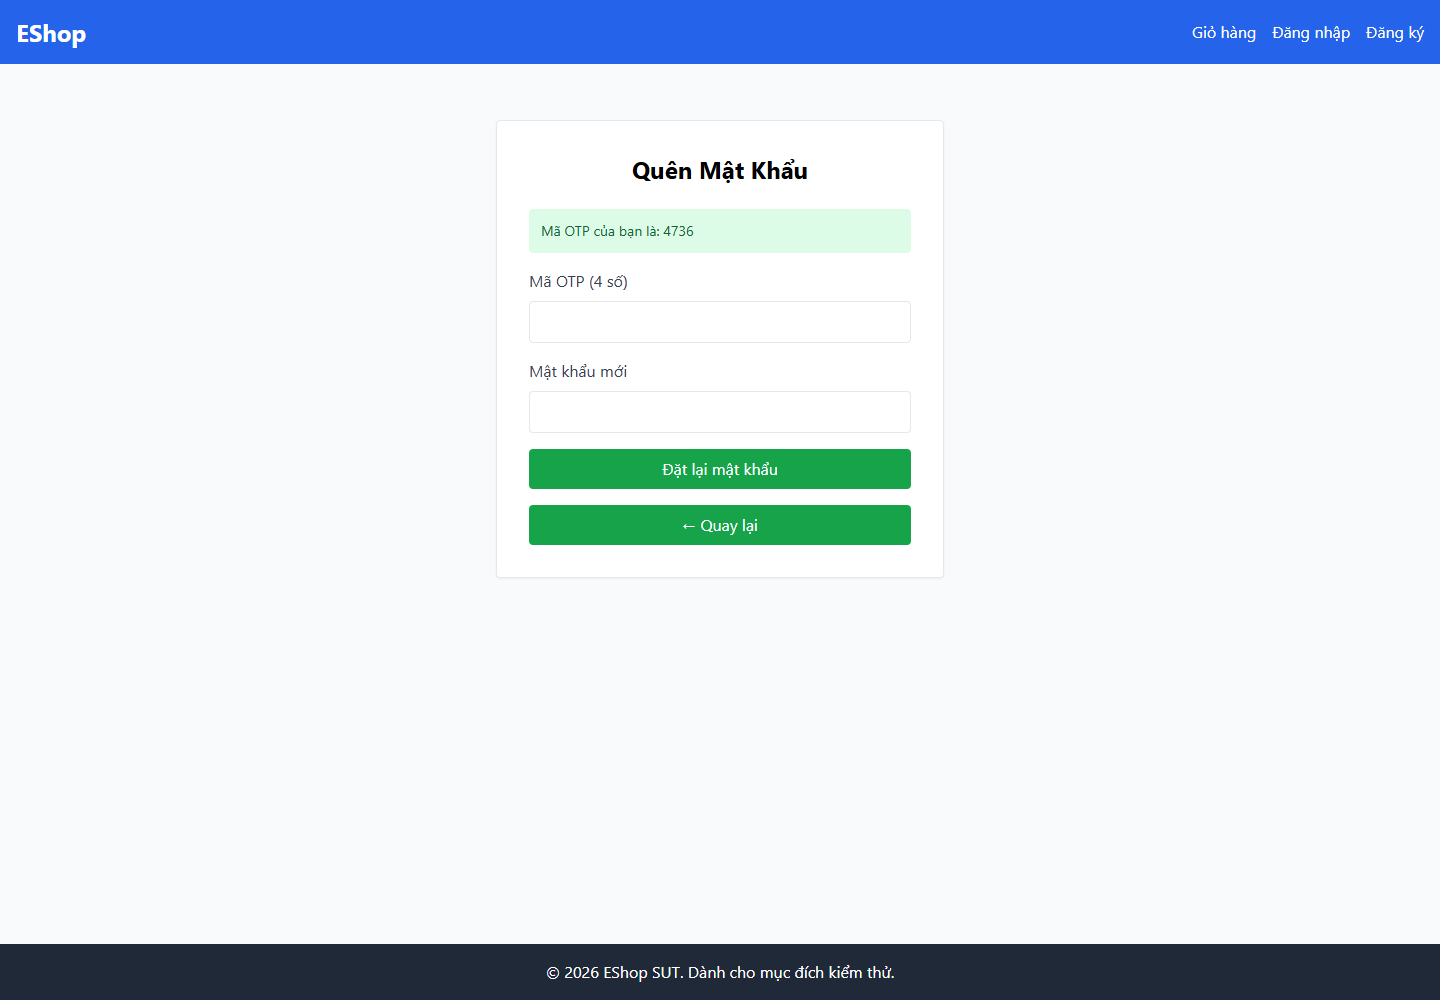
\includegraphics[width=0.82\textwidth]{../../evidence/A/execution/screenshots/A-TC-001.png}
  \caption{A-TC-001 FAIL: SUT phát hành và hiển thị OTP 4 chữ số thay vì 6 chữ số.}
  \label{fig:a-fr03-tc001-fail}
\end{figure}

\begin{figure}[H]
  \centering
  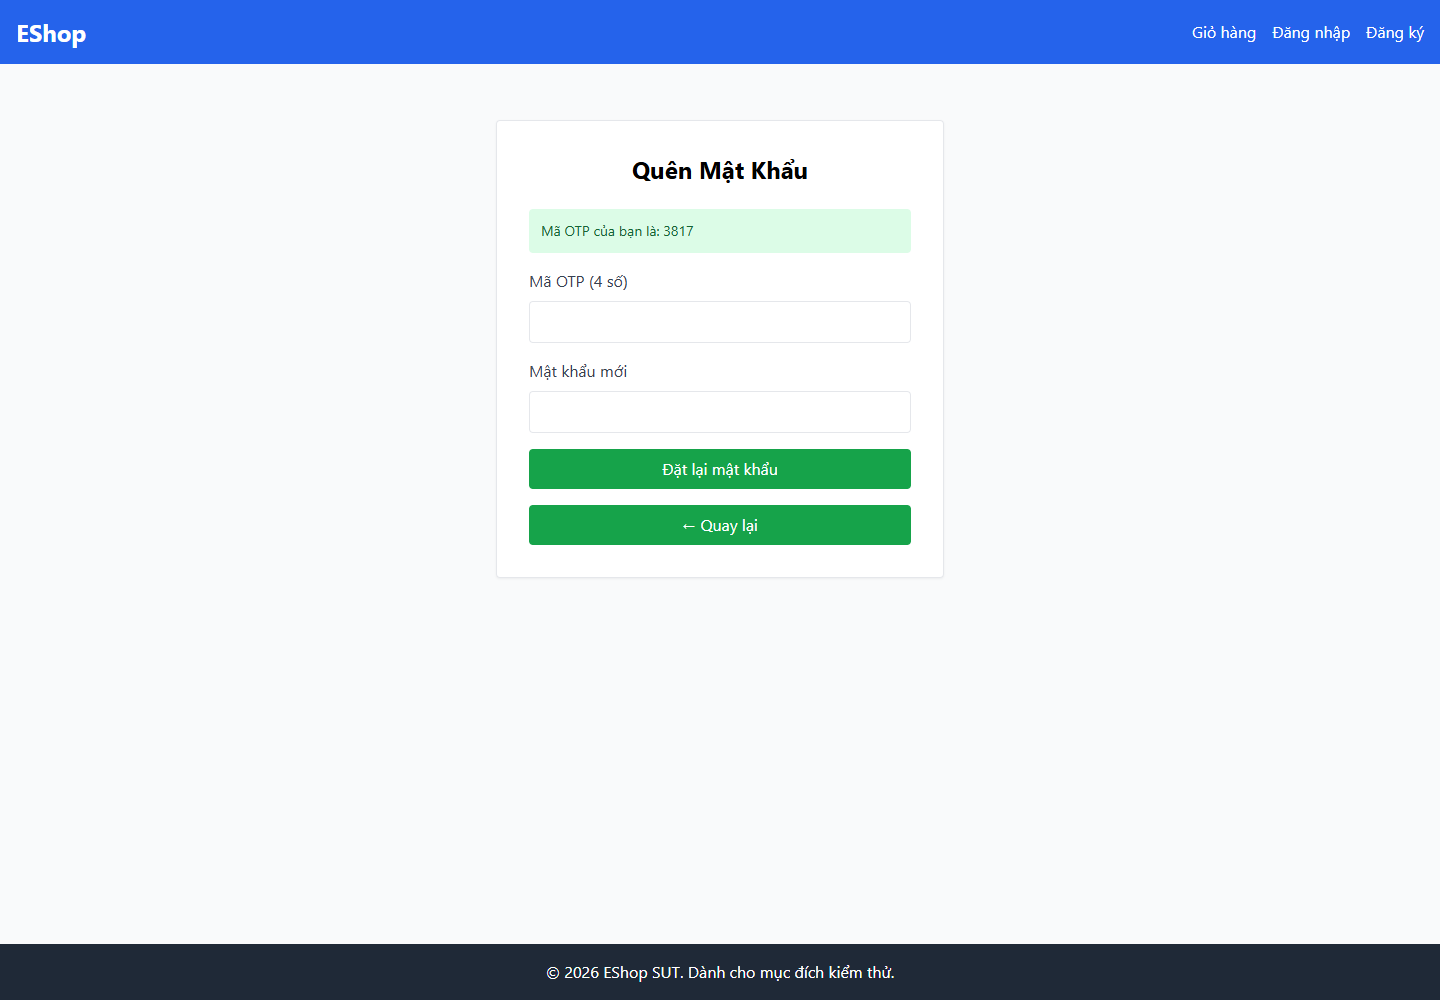
\includegraphics[width=0.82\textwidth]{../../evidence/A/execution/screenshots/A-TC-035.png}
  \caption{A-TC-035 FAIL: Bước 2 thiếu confirm password và required marker.}
  \label{fig:a-fr03-tc035-fail}
\end{figure}

\section{Defect, gap và residual risk}

Tám defect \texttt{A-BUG-001}--\texttt{A-BUG-008} được nhóm theo root cause.
Hai defect Major/High là OTP chỉ có 4 chữ số và thiếu confirm password. Phân tích
gap còn ghi nhận một requirement gap về expiry, bốn implementation gap bổ sung
và một testability gap. Các static finding không bị chuyển thành execution FAIL.

Design traceability bao phủ đủ \texttt{A-R01}--\texttt{A-R14}; tuy nhiên phần
lớn các điểm BVA chưa được thực thi. Residual risk ở mức cao vì chưa xác nhận
reset nominal, OTP lifecycle, password boundary, confirm equality và password
storage qua luồng Web đúng SRS. Sau khi sửa confirm password và triển khai expiry,
cần chạy regression đủ 29 case đang bị chặn.

Ma trận đầy đủ được lưu tại
\path{features/A/07_traceability_matrix.md}; kết luận kỹ thuật và danh sách nội
dung chưa kiểm chứng nằm tại \path{features/A/07_feature_closure.md}.
